\documentclass[twoside,11pt]{article}

% Any additional packages needed should be included after jmlr2e.
% Note that jmlr2e.sty includes epsfig, amssymb, natbib and graphicx,
% and defines many common macros, such as 'proof' and 'example'.
%
% It also sets the bibliographystyle to plainnat; for more information on
% natbib citation styles, see the natbib documentation, a copy of which
% is archived at http://www.jmlr.org/format/natbib.pdf

\usepackage{jmlr2e}
\usepackage{graphicx}
\usepackage{wrapfig}
\usepackage{amsmath}

% Definitions of handy macros can go here

\newcommand{\dataset}{{\cal D}}
\newcommand{\fracpartial}[2]{\frac{\partial #1}{\partial  #2}}

% Short headings should be running head and authors last names

\ShortHeadings{Comparing Naïve Bayes Results}{Brekke, Wall, et. al.}
\firstpageno{1}

\begin{document}
	
	\title{Compared Results of Naïve Bayes Classifiers Across Five Data Sets}
	
	\author{\name Kyle J Brekke \email brekke.kylej@gmail.com \\
		\addr Gianforte School of Computing\\
		Montana State University\\
		Bozeman, MT 59717-2220, USA
		\AND
		\name Ren H. Wall \email renwall@protonmail.ch \\
		\addr Gianforte School of Computing\\
		Montana State University\\
		Bozeman, MT 59717-2220, USA
		\AND
		\name Nicholas J. Rust \email  nicholasrust@protonmail.com \\
		\addr Gianforte School of Computing\\
		Montana State University\\
		Bozeman, MT 59717-2220, USA
		\AND
		\name Alexander Mershon \email alexander.mershon@student.montana.edu \\
		\addr Gianforte School of Computing\\
		Montana State University\\
		Bozeman, MT 59717-2220, USA}
	
	\editor{Kyle J Brekke}
	
	\maketitle
	
	\begin{abstract}%
		In this paper we tested the effect of introducing noise into five data sets used to evaluate the Naïve Bayes algorithm. Our implementation of Naive Bayes utilizes a 10-fold cross validation, and is measured using a paired \textit{t} test. While the introduction of noise to the \textit{breast-cancer-wisconsin}, \textit{house-votes-84}, \textit{glass}, \textit{iris}, and \textit{soybeans} data sets certainly appeared to affect our implementation's accuracy on the data sets, we were unable to make many conclusions as a result of the small size of many of the data sets and low performance of the algorithm in our tests. As such we were unable to produce significant results for all but the \textit{breast-cancer-wisconsin} data set, of which we concluded had support for the hypothesis that the addition of noise would significantly reduce the ability of Naive Bayes to classify items in the data set.
	\end{abstract}
	
	\begin{keywords}
		Machine Learning, Statistics, Naïve Bayes Classifiers
	\end{keywords}
	
	\section{Introduction}\label{sec:introduction}
	
	The purpose of this project is to accurately analyze data sets in a manner which serves as a "gentle introduction" to machine learning. In this report, we will utilize Naïve Bayes Classifiers to categorize data into different classes via the use of training and testing sets. All data sets used in this report are courtesy of the University of California, Irvine, School of Information and Computer Sciences' Machine Learning Repository \citep{Dua:2019}. Particular recognition is provided for the \textit{breast-cancer-wisconsin} data set, produced by Dr. William H. Wolberg \citep{ARTICLE:1, WEBSITE:1}.
	
	The testing of the data will take place in the form of 10-fold cross-validation utilized on two instances of each data set. The first will contain the original, unaltered values of each data set (aside from those removed or discretized during preprocessing), whereas the second sets will have 10\% of their respective features shuffled in order to introduce an additional level of noise to the sets. After experimentation has been conducted on the sets, we will compare the results, and determine whether a significant difference exists between the efficacy of Naive Bayes on the unaltered and altered sets. In general, we expect that the data which has been shuffled will have a significant decrease in efficacy on data sets with few categories, and similar accuracy on data sets with many categories.
	
	\subsection{Hypotheses}\label{subsec:hypotheses}
	\subsubsection{breast-cancer-wisconsin}\label{subsubsec:breast-cancer-wisconsin}
	With 699 entries and only two classes, the breast-cancer-wisconsin data set is larger than most, in conjunction with its 9 attribute categories we hypothesize that the extra noise will have less of an impact on this set than many others.
	
	\subsubsection{glass}\label{subsubsec:glass}
	At 214 entries, 6 classes, and 9 attributes the glass data set is a decent middle-ground. The larger number of classes already makes the data set more difficult to classify, and we hypothesize this will only be exacerbated by increased noise.
	
	\subsubsection{house-votes-84}\label{subsubsec:house-votes-84}
	At 435 entries, 2 classes, and 16 attributes the house votes dataset has one of the larger attribute sets seen in this data sample. We hypothesize that even though the data set has only two classes, the increased number of attributes and noise will lead to a marginal decrease in precision.
	
	\subsubsection{iris}\label{subsubsec:iris}
	With 150 entries, 3 classes, and 4 attributes the iris data set has a comparatively low number of classes and attributes, we hypothesize that since 1/4 of the data is going to be noise, this data set will be extremely affected by the increased noise.
	
	\subsubsection{soybean-small}\label{subsubsec:soybean-small}
	Soybean small has 35 attributes, 47 entries, and 4 classes. With 4/35 of the data being noise, a good number of classes, and a minuscule data set, we hypothesize that soybean-small will see a marginal decrease in performance.
	
	\section{Implementation}\label{sec:implementation}
	
	\subsection{Summary}\label{subsec:summary}
	We started by cleaning the data and splitting each of the five data sets by class into a respective \textit{.csv} file for each class. These are taken in and turned into DataFrames, then split into ten parts. One of each of the ten parts from every DataFrame is then added to a testing set. These testing sets are merged into ten different training and testing set pairs, one testing set is returned as the testing set, and the other four are merged and returned as the training set. These sets are then used to train and test, that data is analyzed and run through the loss functions.
	
	\subsection{Set Creation and 10 Fold Cross Validation}\label{subsec:10-fold-cv}
	Training and testing set creation begins by importing and cleaning the data from a \textit{.csv} file, using the python package \textit{pandas}. The retrieved data is then placed in a DataFrame - a \textit{pandas} object which functions as a table. We then use these DataFrames to conduct our tests using 10-fold cross-validation, an application of the \textit{k}-fold cross-validation method discussed in \textit{Approximate Statistical Tests for Comparing Supervised Classification Learning Algorithms} \citep{Dietterich1997}. The result of our 10-fold cross-validation can be written as such:
	
	\begin{equation}
		k = \frac{1}{10}\sum_{i=1}^{10}c(L = x_j, T = x_i)
	\end{equation}
	
	\begin{enumerate}
		\item Where $c(L,T)$ is the result of our Naive Bayes implementation, $L$ is the training set, and $T$ is the set which the resulting classifier will be tested on.
		\item Where $x_i \in \hat{x} = \{x_1, x_2, ..., x_{10}\}$, given $\hat{x}$ is the set of all entries in the current data set, and $x_1, x_2, ..., x_{10}$ are roughly-equal sized subsets of $\hat{x}$.
		\item Where $x_j$ is the union of all $x \in \hat{x}$, excluding $x_i$.
	\end{enumerate}
	
	In order to implement 10-fold cross validation, the \textit{.csv} files for each class are split into ten parts (by uniform random sampling) and merged with exactly one set from each \textit{.csv} file, creating ten evenly distributed sets which have a proportional amount of each class relative to the original data set. A notable exception to this procedure though, is that the calculated subset scale is rounded down to accommodate datasets which do not have a total number of entries evenly divisible by ten. Any additional entries are added to the first class to ensure no values are dropped. All but one of the subsets are merged together, with each subset being used as the testing set once. This creates ten unique training/testing set pairs, which are then passed on for training and classifying.
	 	
	\subsection{Training and Classifying}\label{subsec:training-and-classifying}
	For our classifier we went with a nested dictionary approach. We accomplished this by first inputting a pandas DataFrame into a method which counts the number of instances of each attribute response for each class and attribute. This cumulative count is put at the leaf of our nested dictionary. The dictionary had the following hierarchy: First key is class, second is either "Probability" or "Attribute," the actual attributes are the keys under "Attribute," this maps to the unique attribute responses, and finally, each unique attribute response maps to the number of times it is counted for that class. The "Probability" key maps to an integer of the elements that are of that specific class.
	
	This is a template for the final nested dictionary we will use for our classification. Next we call our trainer method that goes through and uses the equation for the probability of each attribute response for the given class to give us a fraction we can use to calculate the probability of getting this response in this attribute within this class. Then we go and change the count of each class into the probability of that class, their count divided by the total number of elements. After it finalizes each probability, it puts the finished dictionary into a global dictionary that is used by our classify method.
	
	Our classify method takes in a testing set, which is a pandas DataFrame, iterates through each row and, for each class we saw in our training set, we multiply each attribute response probability together then multiply the class probability and add the total to a tuple list. We then proceed to the next class. After each class is tested for a row, it finds the class with the largest probability and adds that class to the predictions list, which is returned after all the data in the training set has been run. If there was no case of an attribute response in the training set but there is one in the test set, then an amendment is made to the nested dictionary to create a probability with a count of 0 for that response.

	\section{Experimental Approach}\label{sec:experimental-approach}
	
	\subsection{Data Preprocessing}\label{subsec:data-preprosessing}
	There were a number of steps taken for data preprocessing. First, manual modifications were made to a few of the data sets before any cleaning methods were applied. All of the original \textit{.data} files were converted into \textit{.csv} documents. All \textit{.csv} files had a header row containing feature names added as well. Additionally, the ID attribute was removed from the glass and Wisconsin breast cancer data sets, due to its being unnecessary for our purposes.
	
	Of the five total data sets at our disposal, one of them contained missing values in its entries. This required us to develop a method for handling them. We concluded that we would use a 5\% threshold to determine whether entries containing missing values would be imputed, or stricken from the set outright. That is, if the total number of entries containing missing values in a data set was less than 5\% of the total number of entries for that set, then those entries would be removed from it.

	Within the single data set with missing values -- the Wisconsin breast cancer set -- roughly 2.69\% of all entries contained missing values, which was under our selected threshold. As such, all entries with missing values were removed from the Wisconsin breast cancer set during cleaning.
	
	After cleaning was completed, it was necessary for us to modify the \textit{iris} and \textit{glass} data sets to fit our model. Since the data in these sets are real values, they conflicted with our implementation of Naive Bayes as a result of the model being designed for binary and discrete/categorical feature spaces. Our solution to this problem was to categorize each set of attribute values in these data sets into roughly even-sized categories, such that the attributes would be categorized from least to greatest. With this approach, we chose to categorize the \textit{iris} features into six groups, and the \textit{glass} data set into eight groups. Our reasoning for these values was based on loose testing as to what number of categories would yield the greatest classification accuracy in the non-shuffled data sets.

	\subsection{Testing Procedures}\label{subsec:testing-procedures}
	
	Each data set will be tested in two contexts: 1$)$ Using the base values as they are assigned in the processed data sets, and 2$)$ using modified copies of the cleaned data sets which have had values randomly reassigned within 10\% of their respective features.
		
	Once these instances have been tested, we will compare their results using paired \textit{t} tests to evaluate whether our implementation of Naive Bayes is more or less efficient when data is scrambled when compared to the base case. The comparisons we will be making in this report are the results of three loss functions: \textit{error}, \textit{precision}, and \textit{recall}.
	
	\begin{equation}
		error = \frac{c_{01} + c_{10}}{c_{11} + c_{10} + c_{01} + c_{00}}
	\end{equation}
	
	\begin{equation}
	precision = \frac{c_{11}}{c_{11} + c_{10}}
	\end{equation}
	
	\begin{equation}
	recall = \frac{c_{11}}{c_{11} + c_{01}}
	\end{equation}
	
	The values $c_{11}$, $c_{10}$, $c_{00}$, and $c_{01}$ in the above equations are respectively the counts of all true positives, false positives, true negatives, and false negatives which resulted from the classifications conducted.
	
	\textit{Error} is representative of the total number of misclassified entries, relative to the total number of all classified entries. The actual value of \textit{error} indicates the overall ratio of misclassifications in the dataset.
	
	\textit{Precision} indicates how many classifications into a given category where correct. The actual value of \textit{precision} is the ratio of all true positive classifications, relative to all classifications asserted to be positive.
	
	\textit{Recall} represents the number of correct classifications of a given class out of all actual instances of that class in the dataset.
		
	Once the loss functions have been calculated for all classes, they are averaged for their corresponding data sets. We then apply the paired \textit{t} test illustrated in \textit{Approximate Statistical Tests for Comparing Supervised Classification Learning Algorithms} \citep{Dietterich1997}:
	
	\begin{equation}
		t = \frac{\bar{p}\sqrt{10}}{\sqrt{\frac{\sum_{i=1}^{10}(p^{(i)}-\bar{p})^2}{9}}}
	\end{equation}
	
	\begin{enumerate}
		\item Where $\bar{p}$ is the overall average of one of our loss functions in a shuffled data set, subtracted from the average of the same loss function in its corresponding unshuffled data set.
		\item Where $p^{(i)}$ is the difference of an average loss function for a data set $i$, and the corresponding value of its paired shuffled data set.
	\end{enumerate}

	The resulting \textit{t} values we acquire can then be used to determine the significance of any differences we observe between the unaltered and shuffled data sets.
	
	\section{Results}\label{sec:results}
	After running our tests, we acquire a text dump of data which allows us to gleam a wide array if information about our implementation and data sets. 
	
	
	\begin{wrapfigure}{r}{0.55\textwidth}
		\centering
		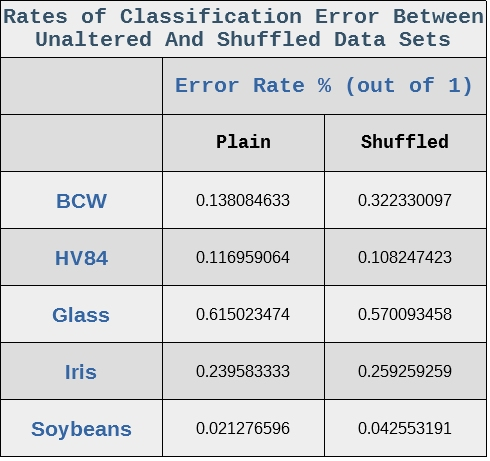
\includegraphics[width=0.55\textwidth]{error_data.jpg}
		\caption{\label{fig:1} Table containing the error rates of our five data sets.}
	\end{wrapfigure}

	Of note, we are able to observe that the lowest performing data set in both the plain and shuffled tests was by far the \textit{Glass} data set with an error rate of around 61.502\% in the plain data tests, and 57.009\% in the shuffled tests. Meanwhile the highest performing data set was the \textit{Soybean} set, with the lowest error rate of roughly 2.128\% in the plain tests, and 4.256\% in the shuffled tests (see \textit{Figure 1}).
	
	We can also observe that two of our five datasets actually \textit{increased} in accuracy after the data was shuffled, though neither seemed to by a particularly major amount. Despite this though, we can also observe marginally stronger trend in the other two loss functions which align with our initial assumptions (see \textit{figures 3} and \textit{4}). \bigbreak
	
	\begin{figure}[!h]
		\centering
		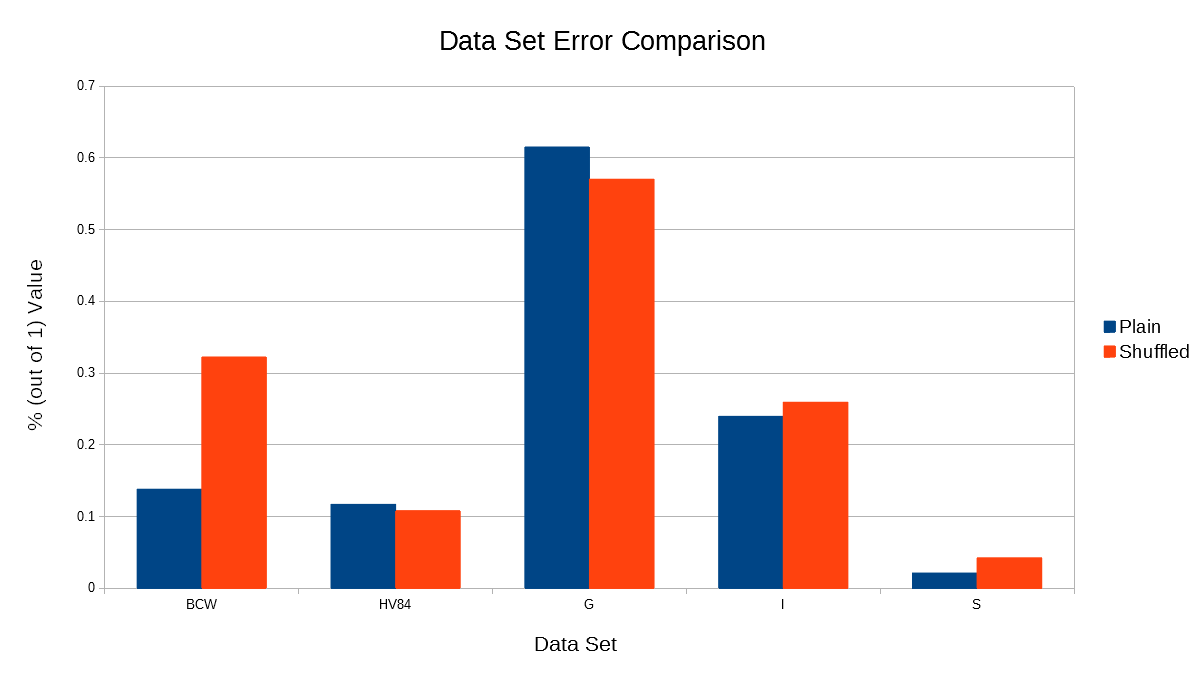
\includegraphics[width=0.9\textwidth]{error_comparison.png}
		\caption{\label{fig:2} Graph comparing the error rates of our five data sets. From left-to-right: Breast Cancer in Wisconsin (BCW), House Votes in 1984 (HV84), Glass (G), Iris (I), and Soybeans (S)}
	\end{figure}
	\begin{figure}[!h]
		\centering
		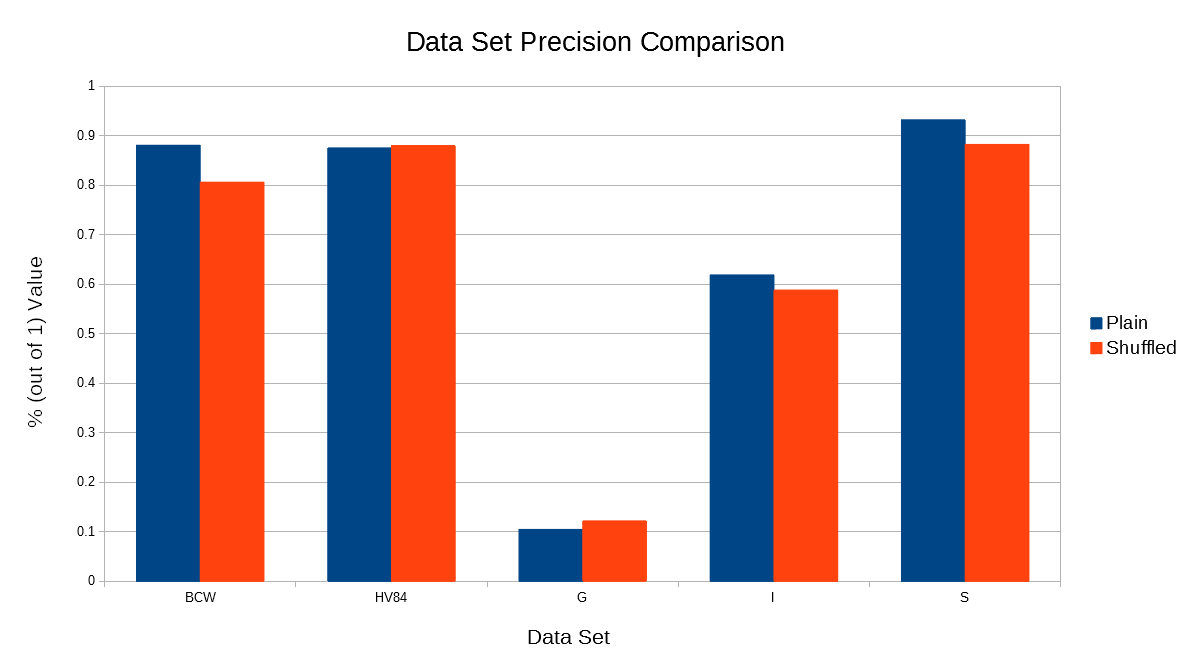
\includegraphics[width=0.9\textwidth]{precision_comparison.png}
		\caption{\label{fig:3} Graph comparing the precision values of our five data sets}
	\end{figure}
	\begin{figure}[!h]
		\centering
		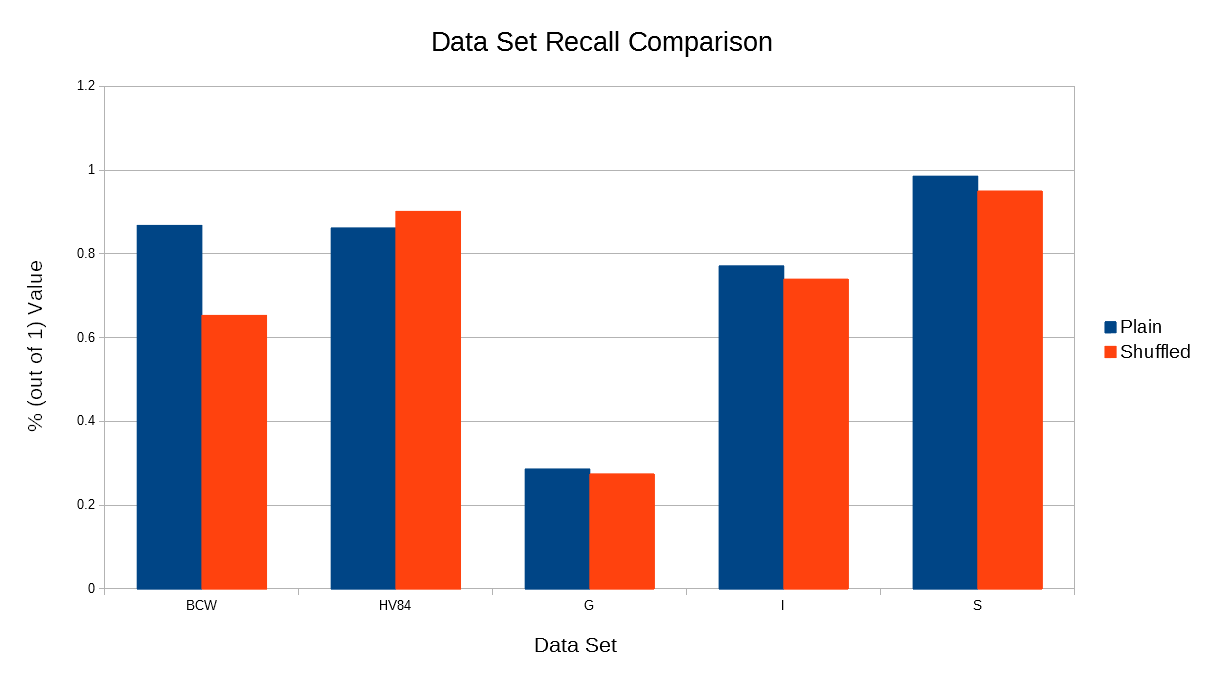
\includegraphics[width=0.9\textwidth]{recall_comparison.png}
		\caption{\label{fig:4} Graph comparing the recall of our five data sets.}
	\end{figure}

	Based off both of the above figures, we have a mildly stronger case for our hypothesis. Despite what we may be able to derive from our findings, we are not able to determine the significance of our data until we evaluate the results of our paired \textit{t} tests.

	\clearpage
	\section{Conclusions}\label{sec:conclusions}
	
	Using the \textit{error} values of our datasets does not allow us to make many statements regarding the affects of adding noise to the dataset. For \textit{breast-cancer-wisconsin}, \textit{house-votes-84}, \textit{glass}, \textit{iris}, and \textit{soybeans}, the \textit{t} values are:
	
	\begin{align*}
		t_{9,.975} &= |-6.90699| = 6.90699 \\
		t_{9,.975} &= 0.40645 \\
		t_{9,.975} &= 0.99174 \\
		t_{9,.975} &= |-0.29689| = 0.29689 \\
		t_{9,.975} &= |-0.55708| = 0.55708 \\
	\end{align*}
	
	Given these values, we are only able to reject the null hypothesis for the \textit{breast-cancer-wisconsin} data set, with 95\% confidence. We are unable to reduce our confidence interval, due to the magnitude of such a reduction. To consider even the second highest \textit{t} value significant would require us to lower our confidence to 60\%, while all other data sets would still be non-significant. As such, we can not make conclusions about any data set aside from the \textit{breast-cancer-wisconsin} set.
	
	Because we are able to consider the results of our experimentation with \textit{breast-cancer-wisconsin} significant, we support the experimental hypothesis that introducing noise to a data set has a measurable effect on the accuracy of Naive Bayes on the set.

	\section{Summary}\label{sec:summary}
	
	 In this report, we utilized Naive Bayes to classify data into different categories through training and testing sets. The sets which we tested on were the \textit{breast-cancer-wisconsin} \citep{ARTICLE:1}, \textit{house-votes-84}, \textit{glass}, \textit{iris}, and \textit{soybeans} datasets from the UCI Machine Learning Repository \citep{Dua:2019}.
	
	The testing of the data took place in the form of 10-fold cross-validation run on two instances of each data set, an unaltered instance and a shuffled instance. After experimentation was complete, we compared the results to determine whether a discernible difference in accuracy arose between the plain and shuffled sets. 
	
	Our initial assumptions led us to believe that the introduction of noise would significantly reduce the efficacy of Naive Bayes on the data sets. However, the results of our paired \textit{t} test did not yield sufficient data to form a conclusion on any set other than the \textit{breast-cancer-wisconson} set. We suspect that this was a result of the relatively small size of the data sets, and the poor performance of the Naive Bayes model during our test. 
	
	From the conclusions we are able to develop, we can affirm that the data supports the experimental hypothesis for the \textit{breast-cancer-wisconsin} set, that the addition of noise reduced the effectiveness of our model significantly.
	
	\newpage
	\vskip 0.2in
	\bibliography{bibliography}
	
\end{document}
